\documentclass[12pt]{article}
\usepackage[english,greek]{babel}
\usepackage[utf8x]{inputenc}
\usepackage{graphicx}
\usepackage{fullpage}
\begin{document}

\title{\selectlanguage{english}Stakeholders Requirements Specification}
\date{\today}
\author{\selectlanguage{english}Javengers}

\maketitle

\tableofcontents

\section{Εισαγωγή}
\subsection{Ταυτότητα-Επιχειρησιακοί Στόχοι}


Ο σκοπός της εργασίας είναι να αναπτυχθεί ένα διαδικτυακό παρατηρητήριο τιμών, το οποίο θα δίνει τη δυνατότητα αναζήτησης προϊόντων σε διάφορα καταστήματα, καθώς επίσης και την εισαγωγή νέων καταχωρήσεων από τους εγγεγραμένους χρήστες. Στο πλαίσιο αυτό, η εφαρμογή μας βασίζεται στη μέθοδο του \selectlanguage{english}crowdsourcing, \selectlanguage{greek}όπου εθελοντές θα καταγράφουν και θα μοιράζονται τις τιμές από διάφορα καταστήματα, μέσω της δικτυακής μας υπηρεσίας. 

\subsection{Περίγραμμα επιχειρησιακών λειτουγιών}

Οι χρήστες στους οποίους απευθύνεται η εφαρμογή μας μπορούν να ομαδοποιηθούν στους ακόλουθες κατηγορίες:
\begin{itemize}
	\item Απλός επισκέπτης: Πραγματοποιεί αναζητήσεις προϊόντων και περιηγείται αξιοποιώντας μια μηχανή αναζήτησης αλλά και πολλαπλά κριτήρια κατηγορποίησης.
	\item Εγγεγραμένος χρήστης: Συνδέεται με τη χρήση ενός λογαριασμού που έχει δημιουργήσει και στη συνέχεια είναι σε θέση να προσθέσει και να αξιολογήσει καταχωρήσεις. Επιπλέον, του δίνεται η δυνατότητα να επικοινωνήσει με το διαχειριστή της σελίδας.  
	\item Διαχειριστής: Συνδέεται με τη χρήση ενός ειδικού λογαριασμού και αλληλεπιδρά με τους εγγεγραμένους χρήστες.
\end{itemize}

\begin{center}
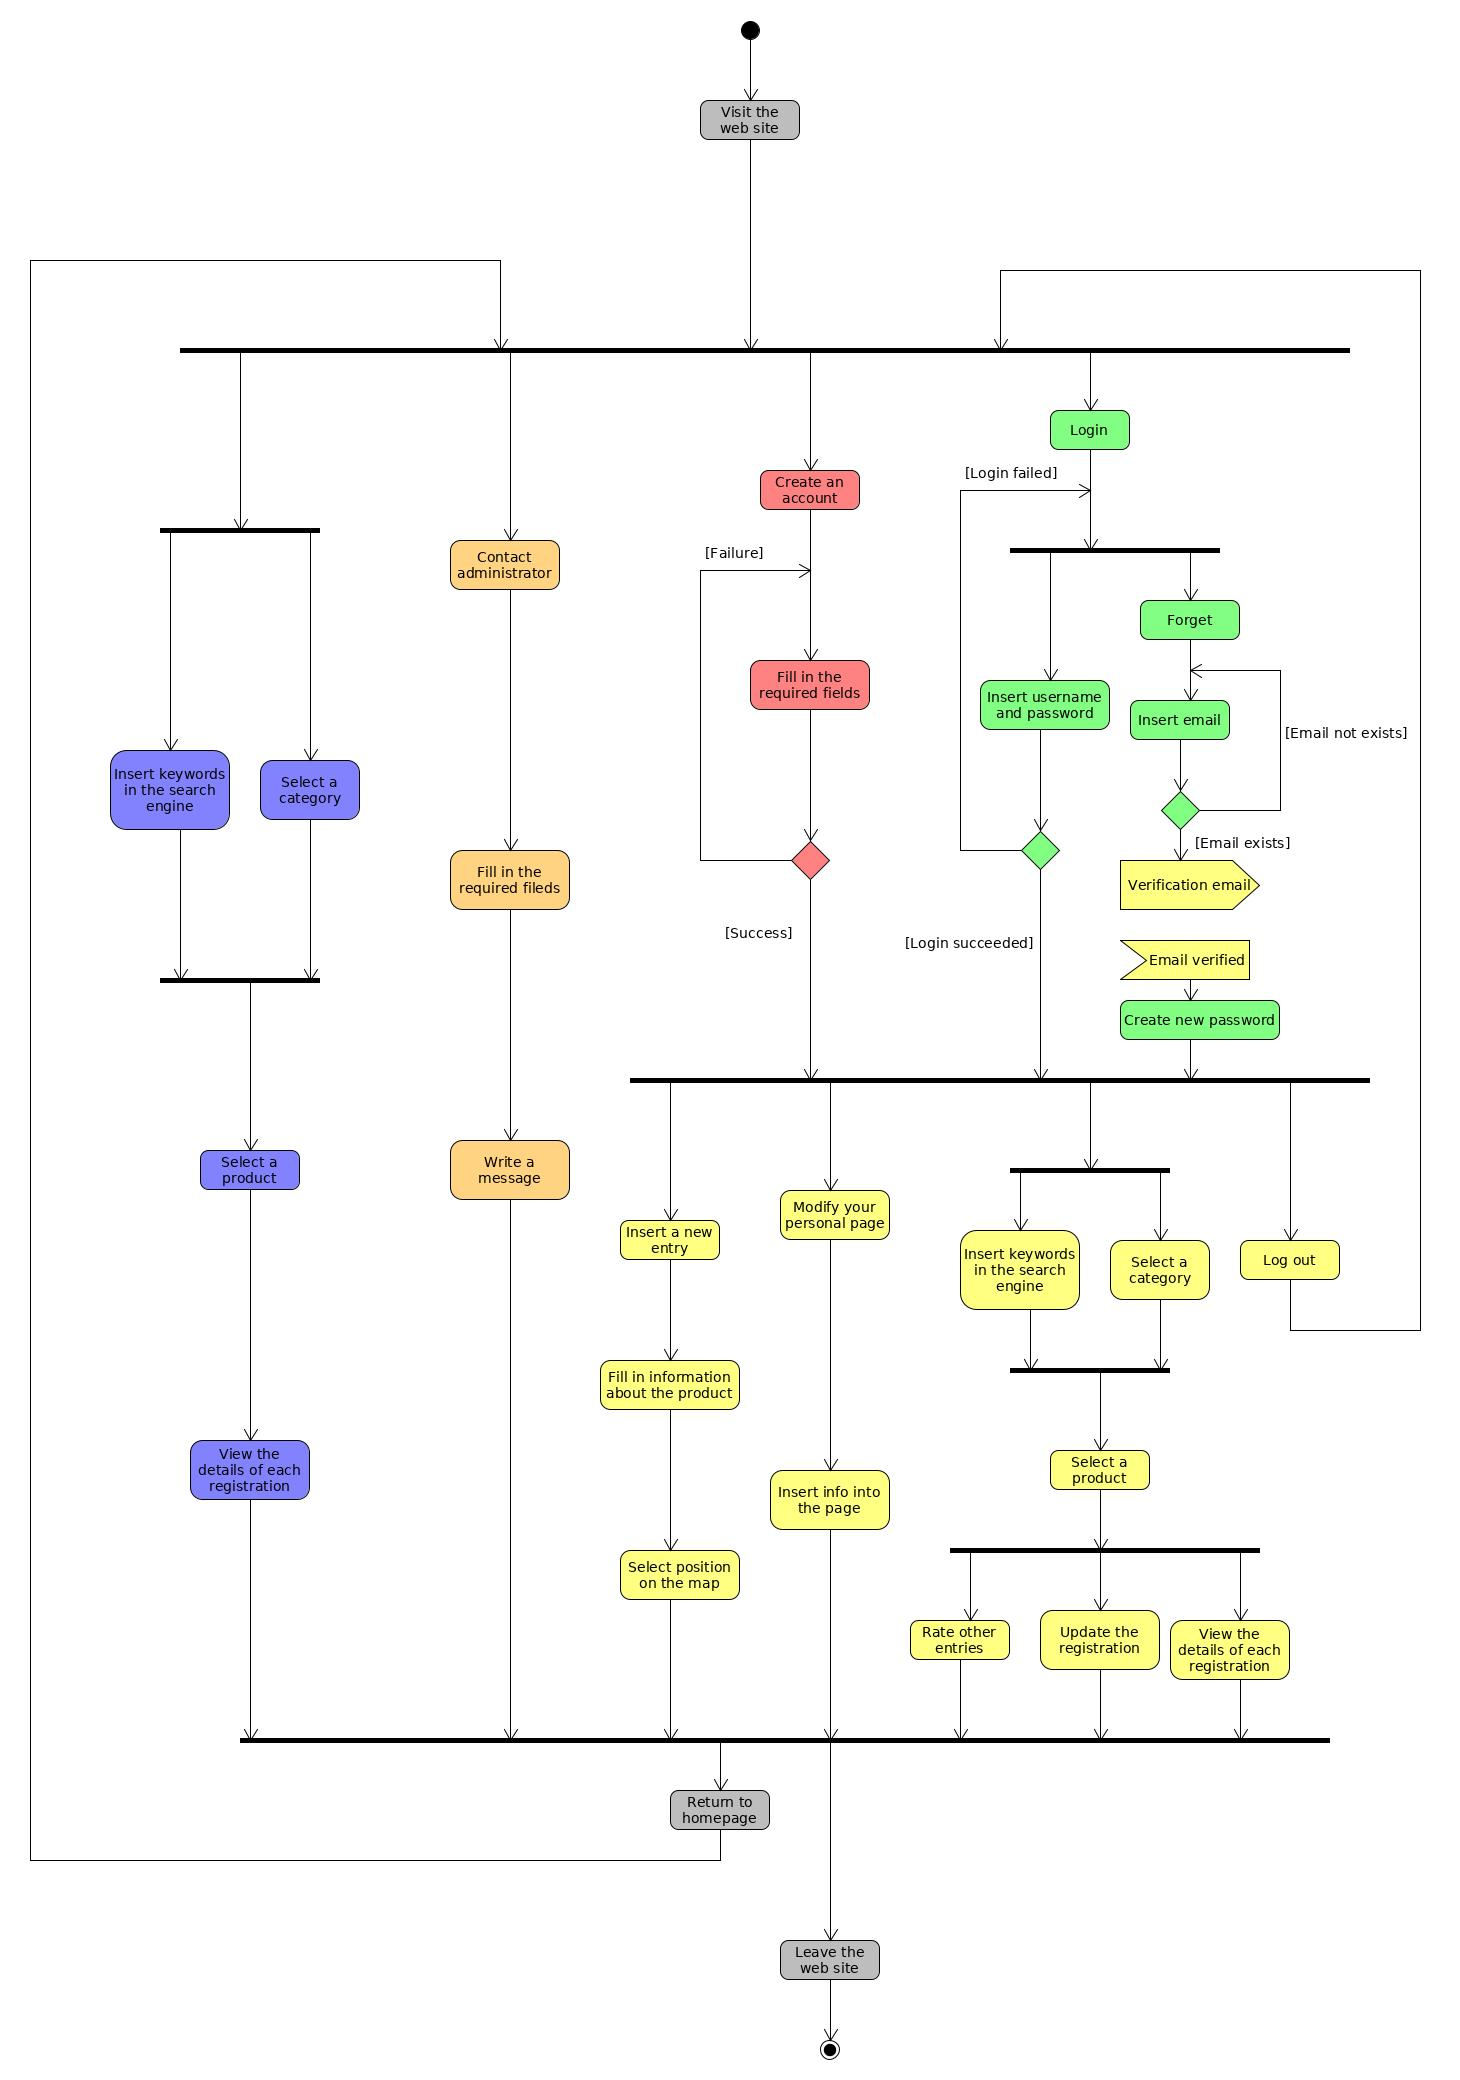
\includegraphics[scale=0.35]{activityDiagram.pdf}
\end{center}

\section{Αναφορές-Πηγές Πληροφοριών}





\subsection{Αναφορές - Πηγές πληροφοριών}



\end{document}

